%----------------------------------------------------------------------------------------
%	PACKAGES AND THEMES
%----------------------------------------------------------------------------------------
\documentclass[aspectratio=169,xcolor=dvipsnames, t]{beamer}
\usepackage{fontspec} % Allows using custom font. MUST be before loading the theme!
\usetheme{SimplePlusAIC}
\usepackage{hyperref}
\usepackage{graphicx} % Allows including images
\usepackage{booktabs} % Allows the use of \toprule, \midrule and  \bottomrule in tables
\usepackage{svg} %allows using svg figures
\usepackage{tikz}
\usepackage{makecell}
\usepackage{wrapfig}
\usepackage{ragged2e}
\usepackage{setspace}
\usepackage{multirow}
\renewcommand{\baselinestretch}{1.0} 
% ADD YOUR PACKAGES BELOW

%----------------------------------------------------------------------------------------
%	TITLE PAGE CONFIGURATION
%----------------------------------------------------------------------------------------
\title[short title]{DEEP ANALYSIS AND PREDICTION OF CHIKUNGUNYA USING ENSEMBLE REGRESSION APPROACH} % The short title appears at the bottom of every slide, the full title is only on the title page
\subtitle{Mémoire présenté en vue d’obtention du diplôme de Master en Ingénierie Informatique\\Parcours :\textbf{ Systèmes et Logiciels en Environnements Distribués}}
\author[MOHAMED EL BACHIR]{MOHAMED EL BACHIR BOUBA NGANADAKOUA\\\textbf{19A666FS}\\( Licence en Informatique )}
\institute[MOHAMED EL BACHIR ( M2SLED / Université de Ngaoundéré )]{
	\centering
	\normalsize{Sous la direction de :}\\[0.2cm]
	\begin{columns}[c]
		\begin{column}{6cm}
			\centering
			\footnotesize{\textbf{Dr. ABBOUBAKAR Hamadjam}\\ \textit{Chargé de Cours \\Université de Ngaoundéré}}
		\end{column}
		\begin{column}{6cm}
			\centering
			\footnotesize{ \textbf{Dr. ZONGO MEYO Epse NDO}\\ \textit{Chargé de Cours \\ Université de Ngaoundéré}}
		\end{column}
	\end{columns}
	\vspace{0.2cm}
	\textbf{Année académique : 2023-2024}}
% Your institution as it will appear on the bottom of every slide, maybe shorthand to save space


\date{\today} % Date, can be changed to a custom date
%----------------------------------------------------------------------------------------
%	PRESENTATION SLIDES
%----------------------------------------------------------------------------------------

\begin{document}
	
	\maketitlepage
	
	\begin{frame}[t]{Plan du travail}
		% Throughout your presentation, if you choose to use \section{} and \subsection{} commands, these will automatically be printed on this slide as an overview of your presentation
		\tableofcontents
	\end{frame}
	
	%------------------------------------------------
	% Section divider frame
	\makesection{Introduction}
	
	%------------------------------------------------
	% Introduction
	\begin{frame}{Introduction}
		\setstretch{1.2}
		\begin{block}{Contexte}
			\justifying
			Le \textbf{2 août 2024} , Le Centre européen de contrôle et de prévention des maladies (\textbf{ECDC}) a indiqué qu’environ \textbf{350 000 cas} de maladie à virus chikungunya (CHIKVD) et plus de \textbf{140 décès} ont été signalés dans le monde en 2024, Ces cas proviennent de 21 pays \textbf{d’Amérique}, \textbf{d’Asie}, \textbf{d’Afrique} et \textbf{d’Europe} \cite{p1}. Au total, plus de \textbf{2 millions} de cas ont été signalés depuis \textbf{2005}~\cite{p2}. 
			\vskip0.5em%
		\end{block}
	\end{frame}
	\begin{frame}
		\begin{figure}
			\centering
			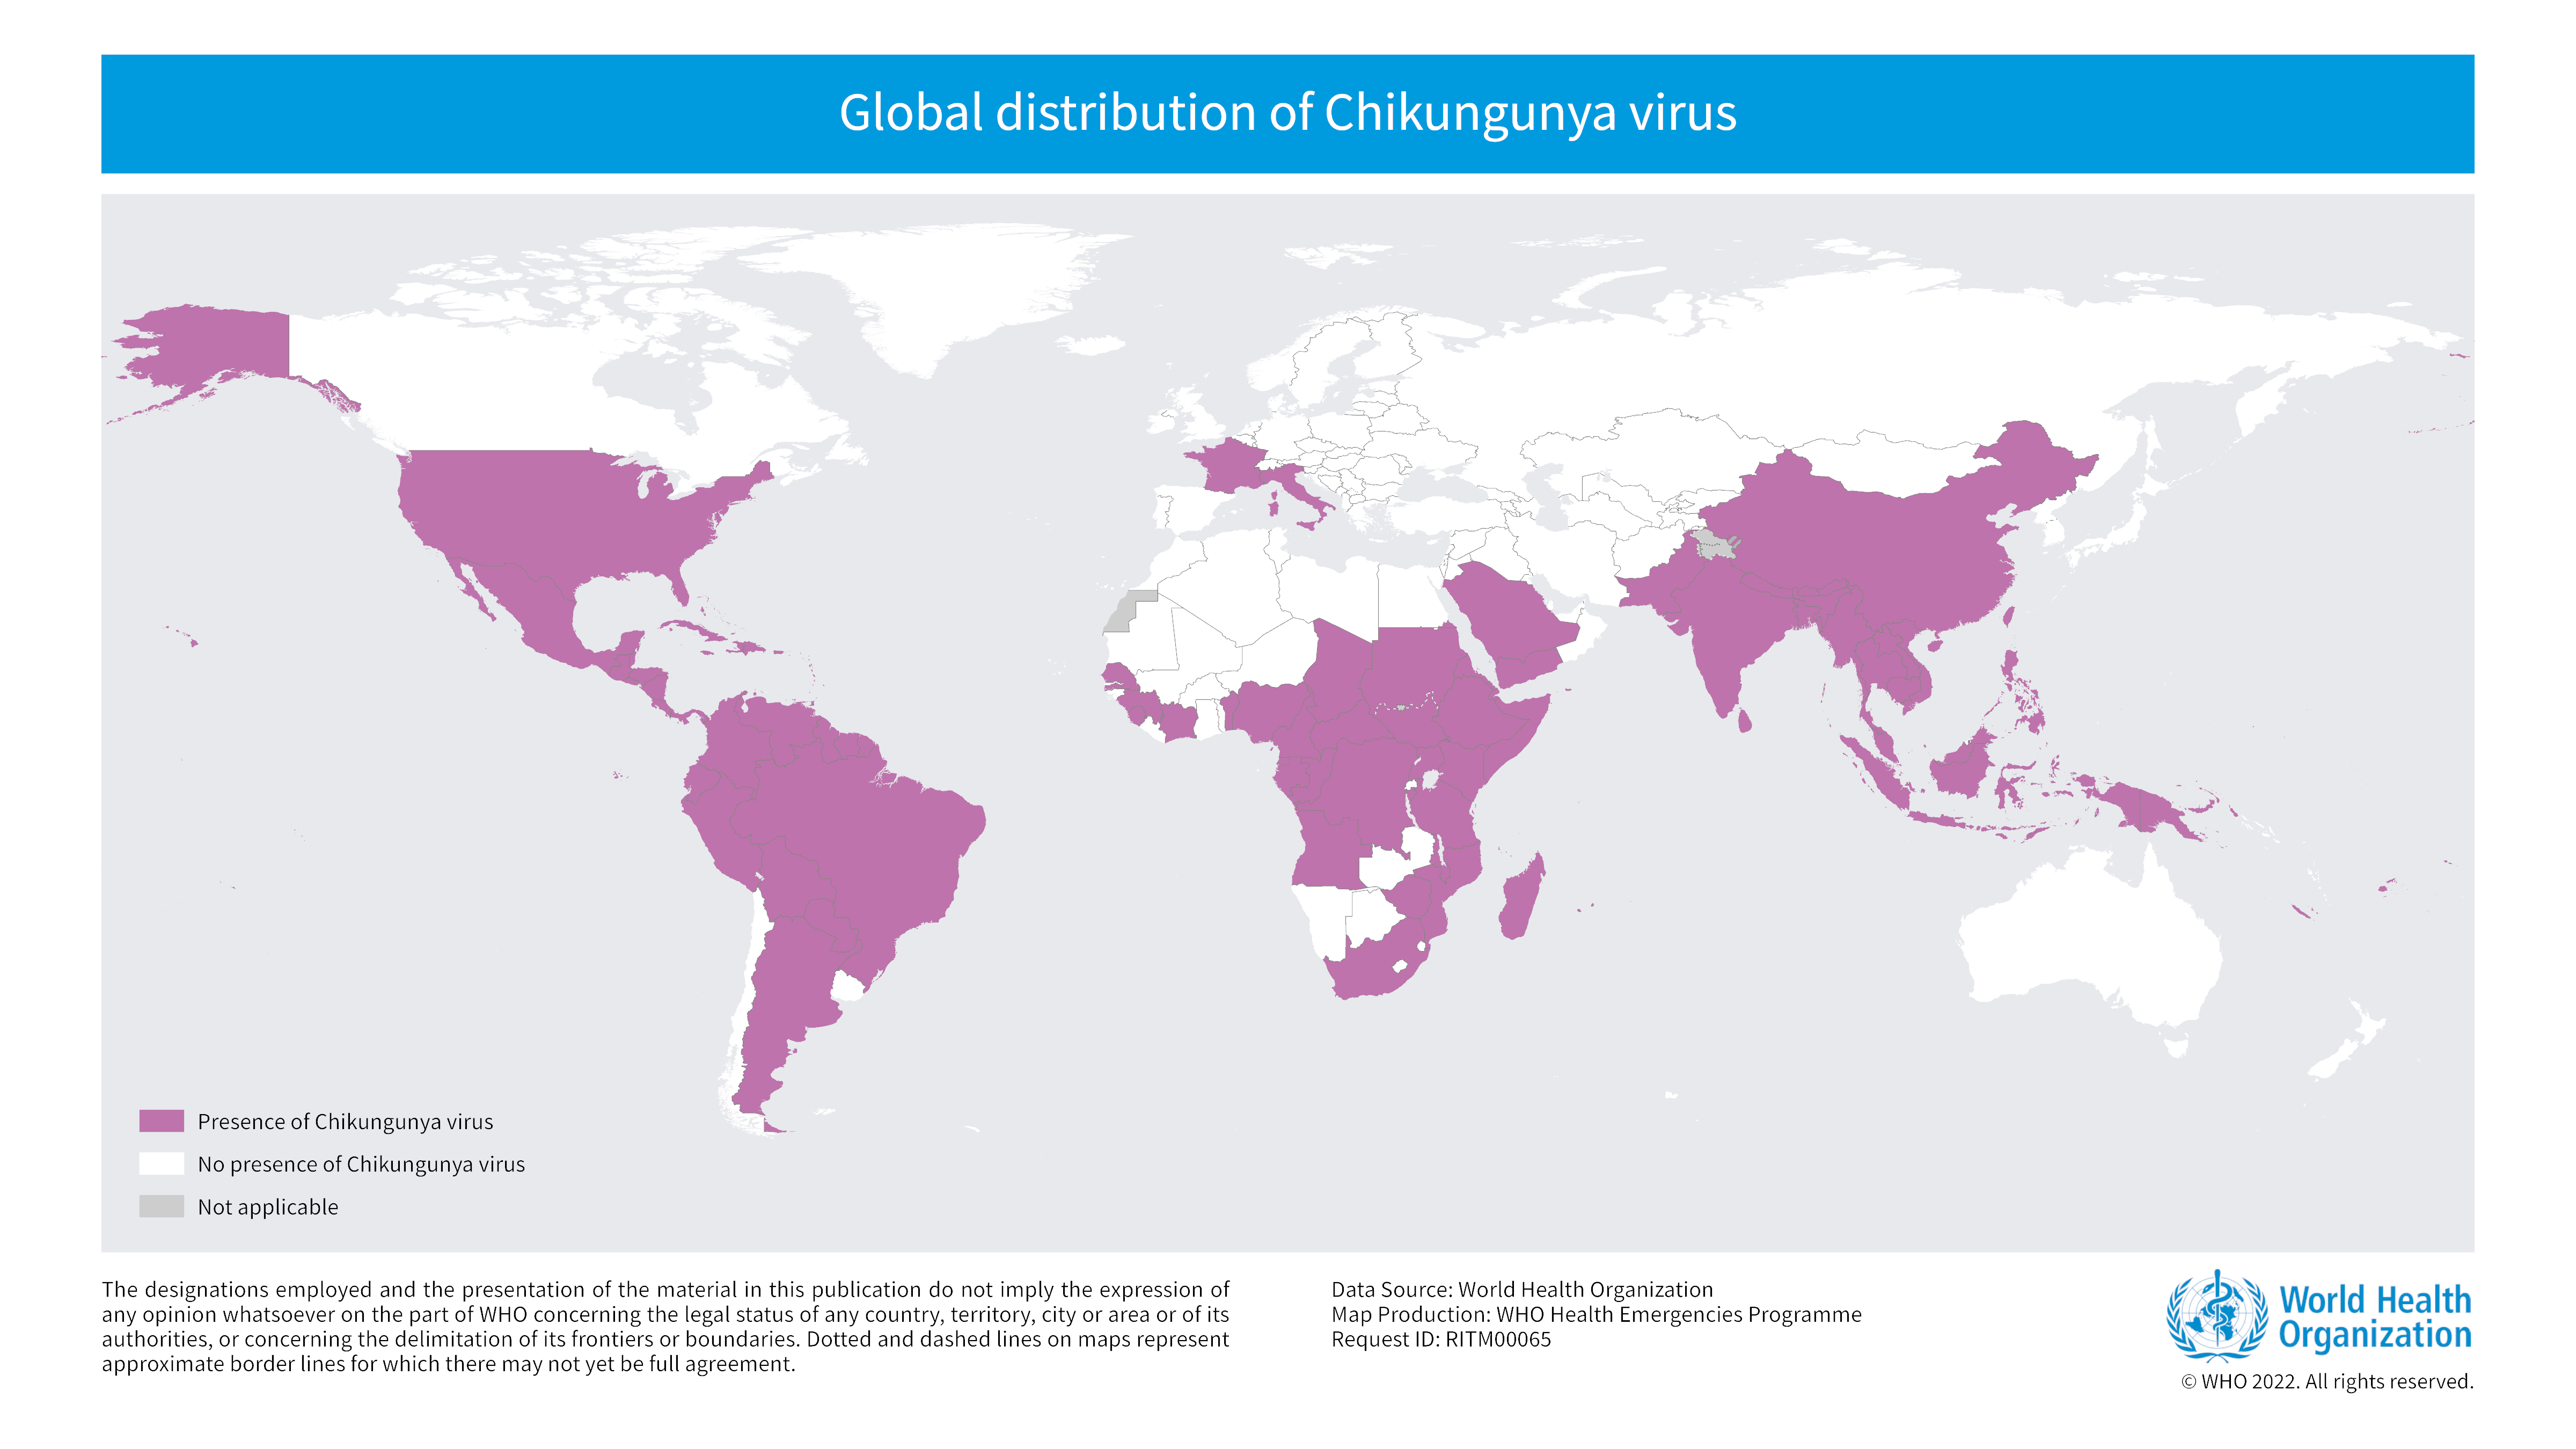
\includegraphics[width=0.9\linewidth]{figures/chikungunya overview.png}
			\caption{la répartion dans le monde  du virus du Chikungunya~\cite{p2}}
			\label{fig:world-chikungunya}
		\end{figure}
	\end{frame}
	
	\begin{frame}{Introduction}
		\justifying
		\setstretch{1.2}
		\qquad Les approches traditionnelles de surveillance épidémiologique se révèlent souvent insuffisantes pour anticiper les épidémies de
		manière proactive (préventive). Ces limites rendent nécessaire le développement de nouvelles méthodes de prédiction et d'analyse, comme l'utilisation de la régression ensembliste , afin d'améliorer la capacité à anticiper aux nouvelles épidémies. \\[1em]
		\pause[2]
		\begin{alertblock}{Problématique}
			\justifying
			Comment prédire et analyser les épidémies du chikungunya en utilisant la régression ensembliste ?
			\vskip0.5em%
		\end{alertblock}
	\end{frame}
	\begin{frame}{Introduction}
		\vskip-1em
		\setstretch{1.2}
		\begin{block}{Objectif général}
			\justifying
			\qquad Développer un modèle prédictif du chikungunya,
			en utilisant des approches de \textbf{régression d'ensemble} dérivées de l'intelligence artificielle, en utilisant les variables climatiques.
			\vskip0.5em%
		\end{block}
		\pause[2]
		\begin{block}{Les objectifs spécifiques de ce travail sont les suivants :}
			\justifying
			\begin{enumerate}
				\item Comprendre les concepts liés au chikungunya et la régression d'ensemble;
				\item Prédire les épidémies de chikungunya en se basant sur les données climatiques et les cas rapportés au Tchad, au Brésil, et au Paraguay ;
				\item Evaluer les performances obtenues dans ces 3 pays.
			\end{enumerate}
			\vskip0.5em%
		\end{block}
	\end{frame}
	
	%------------------------------------------------
	% Section divider frame
	\makesection{Vue d'ensemble sur le chikungunya et l'apprentissage d'ensemble}
	
	%------------------------------------------------
	% Lists
	\begin{frame}{Vue d'ensemble sur le chikungunya}
		\setstretch{1.2}
		\justifying
		\textbf{\large{Définitions et origines}}\\[0.2cm]
		\qquad Le \textbf{chikungunya} est une maladie transmise principalement par les moustiques \textbf{femelles} \textit{Aedes aegypti} et \textbf{Aedes albopictus}.
		elle est décrite pour la première fois en \textbf{1952} lors d'une épidémie dans le sud de la \textbf{Tanzanie}. Le nom vient d'un mot de la langue \textit{Makonde}, parlée dans le sud-est de la Tanzanie et le nord du Mozambique, qui signifie "\textit{ce qui se plie}".\\[0.2cm]
	\end{frame}
	\begin{frame}{Vue d'ensemble sur le chikungunya}
			\begin{figure}[!h]
				\begin{center}
					%taille de l'image en largeur
					%remplacer "width" par "height" pour régler la hauteur
					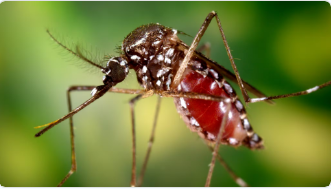
\includegraphics[width=7cm]{figures/moustique}
				\end{center}
				%légende de l'image
				\caption{Le moustique \textit{Aedes aegypti }plein de sang~\cite{p3}}
			\end{figure} 
	\end{frame}
	\begin{frame}{Vue d'ensemble sur le chikungunya}
		\setstretch{1.2}
		\begin{columns}
			\begin{column}{0.45\textwidth}
%			  \colheader{Heading}
				\justifying
			    Le \textbf{CHIKV} (Chikungunya Virus) se transmet selon deux cycles différents :
			    \begin{itemize}
			    	\item \textbf{Cycle urbain}: transmission de l'homme au moustique.
			    	\item \textbf{Cycle sylvatique}: transmission de l'animal au moustique, puis à l'homme.
			    \end{itemize}
			\end{column}
			\begin{column}{0.45\textwidth}  %%<--- here
%			    \colheader{Heading}
			    \begin{figure}
			    	\centering
			    	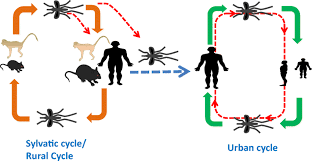
\includegraphics[width=1\textwidth]{figures/trans}
			    	%\begin{center}
			    	\caption{mode de transmission du Chikungunya \cite{p4}}
			    	%\end{center}
			    \end{figure}
			\end{column}
		\end{columns}
	\end{frame}
	\begin{frame}{Vue d'ensemble sur le chikungunya}
		\justifying
		\setstretch{1.2}
		\textbf{\large{Symptômes}}\\[0.2cm]
		\qquad Chez les patients symptomatiques, la maladie se déclare généralement \textbf{4 à 8 jours} après la \textbf{piqûre} d'un\textbf{ moustique infecté}. Elle se caractérise par une brusque \textbf{poussée de fièvre}, souvent accompagnée de \textbf{fortes douleurs articulaires}. Les douleurs articulaires durent généralement quelques jours, mais peuvent être prolongées et durer des semaines, des mois, voire des années.\\[0.2cm]
%		\pause[2]
%		\textbf{\large{Méthodes de contrôle}}\\[0.2cm]
%		\qquad La prévention de l'infection en évitant les piqûres de moustiques est la \textbf{meilleure protection}
	\end{frame}
	\begin{frame}{Impact du chikungunya}
		\setstretch{1.2}
		\begin{columns}
			\begin{column}{0.5\textwidth}
				\colheader{\large Au cameroun}
				\justifying
				\quad En \textbf{2006}, plus de \textbf{400} épidémie de type dengue ont été signalés à \textbf{Kumbo} (région du Nord-Ouest du Cameroun).
				Bien que les investigations aient été menées un an après cette dernière épidémie, les résultats suggèrent une circulation récente du \textbf{CHIKV} dans trois villages de \textbf{Kumbo} (Cameroun occidental).
			\end{column}
			\begin{column}{0.45\textwidth}  %%<--- here
				%			    \colheader{Heading}
				\vskip-2em
				\begin{figure}
					\centering
					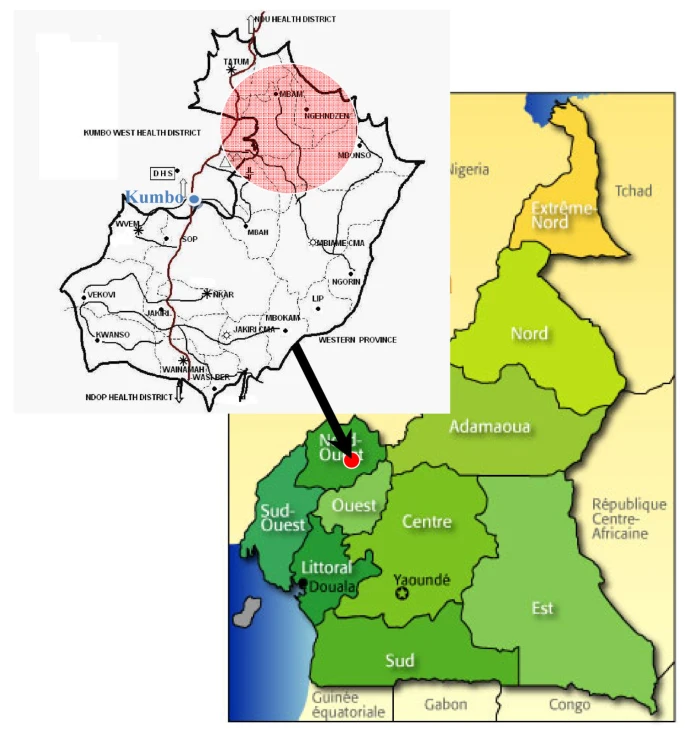
\includegraphics[width=0.6\textwidth]{figures/chikvcameroon}
					%\begin{center}
					\caption{zone d’impact du CHIKV dans la region du Nord Ouest~\cite{p6}}
					%\end{center}
				\end{figure}
			\end{column}
		\end{columns}
	\end{frame}
	\begin{frame}{Impact du chikungunya}
		\setstretch{1.2}
		\begin{columns}
			\begin{column}{0.5\textwidth}
				\colheader{\large Au Tchad}
				\justifying
				\quad Le 3 Septembre 2020, dans le rapport de \textbf{OMS} (Organisation Mondiale de la Santé) \textbf{927} cas ont été notifiés, tous pris en charge en ambulatoire, sans aucun décès. À cette date, le cumul atteignait\textbf{ 13 488} cas, toujours sans décès, avec de nouveaux cas suspects signalés dans les régions  \textbf{OuadaÏ},\textbf{Sila} et \textbf{Wadi Fira}.
			\end{column}
			\begin{column}{0.45\textwidth}  %%<--- here
				%			    \colheader{Heading}
				\vskip-2em
				\begin{figure}
					\centering
					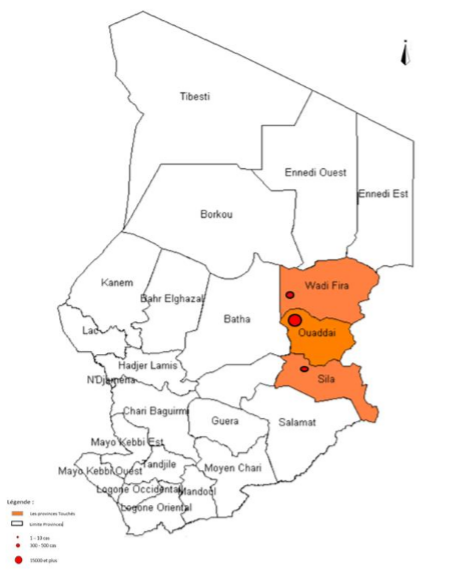
\includegraphics[width=0.6\textwidth]{figures/chadmap}
					%\begin{center}
					\caption{Region infecté au Tchad~\cite{p7}}
					%\end{center}
				\end{figure}
			\end{column}
		\end{columns}
	\end{frame}
	\begin{frame}{Impact du chikungunya}
		\setstretch{1.2}
		\begin{columns}
			\begin{column}{0.5\textwidth}
				\colheader{\large Au Brésil}
				\justifying
				\quad le Brésil, notamment dans l'État de Minas Gerais avec \textbf{395} cas pour 100 000 habitants. Depuis son introduction au Brésil en 2014, avec\textbf{ 3,6 millions} de cas signalés à la \textbf{PAHO} (Pan American Health Organization), la maladie s'est déplacée du Nord-Est vers le Sud-Est.
			\end{column}
			\begin{column}{0.45\textwidth}  %%<--- here
				%			    \colheader{Heading}
				\vskip-2em
				\begin{figure}
					\centering
					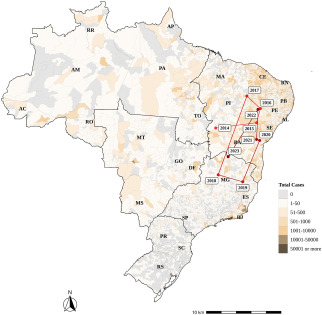
\includegraphics[width=0.6\textwidth]{figures/map_cases_brazil}
					%\begin{center}
					\caption{Carte des épicentres des cas de chikungunya au brésil~\cite{p8}}
					%\end{center}
				\end{figure}
			\end{column}
		\end{columns}
	\end{frame}
	\begin{frame}{Impact du chikungunya}
		\setstretch{1.2}
		\begin{columns}
			\begin{column}{0.5\textwidth}
				\colheader{\large Au Paraguay}
				\justifying
				\quad Des infections autochtones ont été détectées au \textbf{Paraguay} en 2013 et le CHIKV a été détecté dans le pays chaque année depuis cette date toutes associées aux mois d'été. Du 2 octobre 2022 au 10 avril 2023, un total de \textbf{118 179 }infections suspectes et confirmées ont été signalées et 46 décès.
			\end{column}
			\begin{column}{0.45\textwidth}  %%<--- here
				%			    \colheader{Heading}
				\vskip-2em
				\begin{figure}
					\centering
					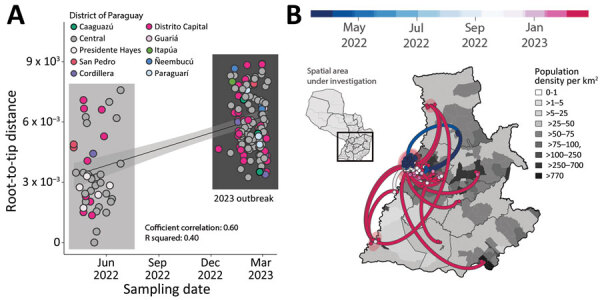
\includegraphics[width=1\textwidth]{figures/paraguay_region_cases}
					%\begin{center}
					\caption{Cas de chikungunya déclarés chaque semaine au paraguay~\cite{p9}}
					%\end{center}
				\end{figure}
			\end{column}
		\end{columns}
	\end{frame}
	\begin{frame}{Concepts sur l'apprentissage d'ensemble}
		\begin{figure}
			\centering
			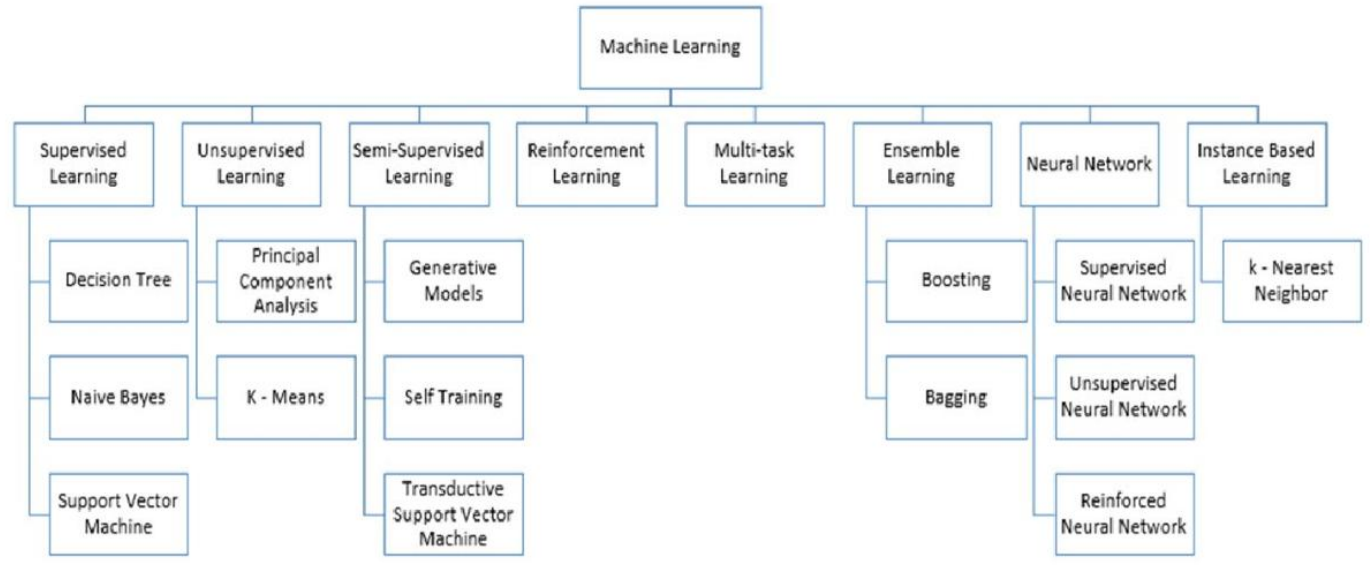
\includegraphics[width=0.9\linewidth]{figures/machineLearningType}
			\caption{Structure arborescente du machine learning ~\cite{p5}}
			\label{fig:world-chikungunya}
		\end{figure}
	\end{frame}
	\begin{frame}{Concepts sur l'apprentissage d'ensemble}
		\justifying
		\setstretch{1.2}
		\begin{block}{Définition}
			L'\textbf{apprentissage d'ensemble} est une technique d'apprentissage automatique qui regroupe deux ou plusieurs apprenants (par exemple, des \textbf{modèles de régression} , des \textbf{réseaux neuronaux} ) afin de produire de \textbf{meilleures prédictions}.
		\end{block}
		\pause[2]
		\begin{block}{ }
			Elle repose sur le principe selon lequel une collectivité d'apprenants produit une plus grande précision globale qu'un apprenant individuel, de même utilisé pour réduire la \textbf{variance} et diminuuer le \textbf{biais}.
		\end{block}
%		{\\[0.2cm]Elle repose sur le principe selon lequel une collectivité d'apprenants produit une plus grande précision globale qu'un apprenant individuel.}
%		\qquad Les \textbf{systèmes d'ensemble} sont développés pour réduire la variance et améliorer la précision des décisions automatisées, ces systèmes se sont avérés efficaces et polyvalents dans divers domaines.\\[0.2cm]
%		\textbf{\large{Définition}}\\[0.2cm]
%		\qquad L'\textbf{apprentissage par ensemble} est une méthode dans laquelle plusieurs \textbf{modèles} sont créés et combinés de manière stratégique pour améliorer la performance et la robustesse dans la résolution d'un problème.
	\end{frame}
	\begin{frame}{Concepts sur l'apprentissage d'ensemble}
		\setstretch{1.2}
		\begin{columns}
			\begin{column}{0.55\textwidth}
				\quad\colheader{\large Type de modèle d'ensemble}
				\begin{itemize}
					\justifying
					\item Les méthodes \textbf{parallèle} : entraînent chaque apprenant de base indépendamment des autres.
					\pause[2]
					\item Les méthodes \textbf{séquentielles }: forment un nouvel apprenant de base de manière à minimiser les erreurs commises par le modèle précédent formé à l'étape précédente.
				\end{itemize}
			\end{column}
			\begin{column}{0.45\textwidth}  %%<--- here
				%\colheader{Heading}
				\vskip-2em
				\begin{figure}[h!]
					\centering
					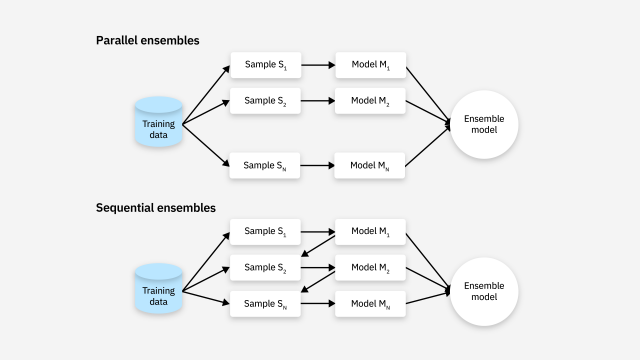
\includegraphics[width=1\textwidth]{figures/type_model_ensemble}
					\caption{Type de modèle d'ensemble~\cite{p10}}
					\label{fig:typemodelensemble}
				\end{figure}
			\end{column}
		\end{columns}
	\end{frame}
	
	\begin{frame}{Concepts sur l'apprentissage d'ensemble}
		\setstretch{1.2}
		\vskip-1em
		Comment les méthodes d'ensemble combinent-elles les apprenants de base pour former un apprenant final ?
		\pause[2]
		\begin{columns}
			\begin{column}{0.5\textwidth}
				\quad\colheader{\large Bagging}
				\justifying
				\begin{figure}[h!]
					\centering
					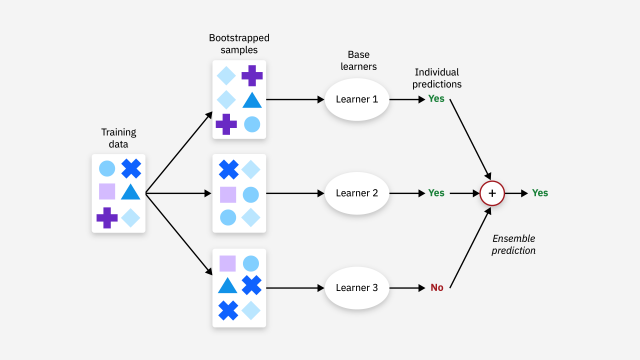
\includegraphics[width=1\linewidth]{figures/Bagging}
					\vskip-1em
					\caption{Bagging~\cite{p10}}
					\label{fig:bagging}
				\end{figure}
			\end{column}
			\begin{column}{0.5\textwidth}  %%<--- here
				\pause[3]
				\colheader{Boosting}
				\begin{figure}[h!]
					\centering
					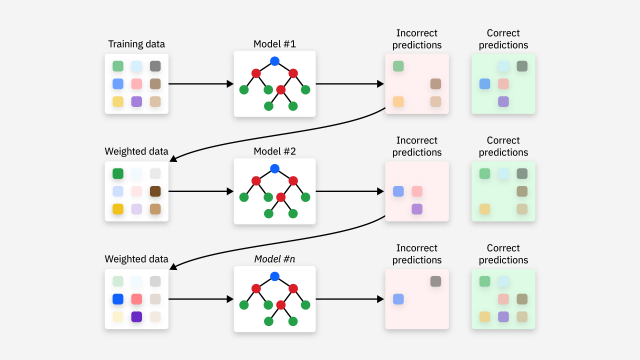
\includegraphics[width=1\linewidth]{figures/Boosting}
					\vskip-1em
					\caption{Boosting~\cite{p10}}
					\label{fig:boosting}
				\end{figure}
				
			\end{column}
		\end{columns}
	\end{frame}
	%------------------------------------------------
	% Section divider frame
	\makesection{l'état de l'art}
	
	%------------------------------------------------
	% Lists
%	Nous avons utilisé la  pour 
	\begin{frame}{l'état de l'art}
		\vskip-1.5em
		\begin{block}{Travaux connexes}
			\justifying
			\setstretch{1.2}
			Dans ~\cite{p11}, prévision de la dengue dans les villes brésiliennes basée sur l'apprentissage automatique à l'aide de variables épidémiologiques et météorologiques
			\begin{itemize}
				\item \textbf{Méthode} :
					\begin{itemize}
						\item algorithme de machine learning (random forests, naive model, gradient boosting regression, a feed-forward neural network ou support vector regression)
						\item méthode du feature selection
					\end{itemize}
				\item \textbf{Résultat} : le modèle \textbf{random forests} était le plus performant
				\item \textbf{Limites} : non utilisation des modèles d'ensemble et aussi elle est basée sur les cas de Dengue
			\end{itemize}
		\end{block}
%		L'\textbf{apprentissage par ensemble} est une méthode dans laquelle plusieurs \textbf{modèles} sont créés et combinés de manière stratégique pour améliorer la performance et la robustesse dans la résolution d'un problème spécifique d'intelligence computationnelle.\\[0.2cm]
%		
%		\textbf{\large{principes de fonctionnement}}\\[0.2cm]
%		Les \textbf{systèmes d'ensemble} sont inspirés par notre pratique quotidienne de consulter divers \textit{experts} avant de prendre des décisions importantes, comme consulter plusieurs médecins avant une opération ou lire des avis avant un achat. Cette approche vise à augmenter notre confiance dans la décision finale en combinant différentes opinions.
	\end{frame}
	\begin{frame}{l'état de l'art}
		\vskip-1em
		\begin{block}{Travaux connexes}
			\justifying
			\setstretch{1.2}
			Dans \cite{p12}, prédiction de la maladie de la dengue basée sur l'apprentissage automatique d'ensemble avec des modèles d'élévation de la performance et de la précision
			\begin{itemize}
				\item \textbf{Méthode} : technique d'apprentissage automatique d'ensemble dans des intégrations hybrides
				\item \textbf{Résultat} : identifier les caractéristiques associées à la propagation de la maladie de la dengue et obtenir de meilleures performances
				\item \textbf{Limites} : utilisation des méthodes hybrides et aussi prediction des caractéristique uniquement
			\end{itemize}
		\end{block}
	\end{frame}
	%------------------------------------------------
	% Section divider frame
	\makesection{Matériel et méthodes}
	%------------------------------------------------
	% Highlight boxes
%	\begin{frame}{Matériel et méthodes}
%		\begin{columns}
%			\begin{column}{0.5\textwidth}
%				\quad\colheader{\large Matériel Physique}
%				\justifying
%				\begin{itemize}
%					\item \textbf{Processeur :} Intel(R) Celeron(R) CPU N2840, 2.16GHz, 4 cœurs
%					\item \textbf{Mémoire RAM :} 4 Go
%					\item \textbf{Stockage :} HDD 250 Go
%					\item \textbf{Système d'exploitation :} Windows 10
%					\item \textbf{Carte graphique :} Intel HD Graphics
%				\end{itemize}
%			\end{column}
%			\pause[2]
%			\begin{column}{0.5\textwidth}  %%<--- here
%				\pause[2]
%				\colheader{Matériel Logiciel}
%				
\includegraphics[width=1\linewidth]{figures/tools}
%			\end{column}
%		\end{columns}
%	\end{frame}
	\begin{frame}{Méthodes de collecte des données}
		\begin{columns}
			\begin{column}{1\textwidth}
				\vskip-3em
				\quad\colheader{\large Données épidémiologiques}
				Les données utilisées dans cette étude proviennent de diverses sources fiables.
				\pause[2]
				\begin{itemize}
					\justifying 
					\item Pour le \textbf{Tchad} : les données épidémiologiques ont été extraites d'un rapport OMS lors de l'émergence du Chikungunya en \textbf{2020}. Ce dataset couvre la période allant du \textit{12 août 2020} au \textit{10 novembre 2020}
					\pause[3]
					\item Concernant le \textbf{Brésil} : les données ont été recueillies à partir du site de mendeley. Cet ensemble de données présente des informations cliniques, \textbf{sociodémographiques} et de laboratoire relatives aux patients confirmés atteints de \textit{dengue} et de \textit{chikungunya}. Il couvre la période de \textbf{2013} à \textbf{2020}, mais pour cette thèse, nous avons restreint notre analyse à l'intervalle de \textbf{2013} à \textbf{2017}.
					\pause[4]
					\item Pour le \textbf{Paraguay} : les données ont été collectées via le site de la PAHO , qui rapporte les cas de Chikungunya en temps réel, avec des enregistrements hebdomadaires variant entre 2013 et 2017.
				\end{itemize}
			\end{column}
		\end{columns}
	\end{frame}
	\begin{frame}{Méthodes de collecte des données}
		\begin{columns}
			\begin{column}{1\textwidth} 
				\vskip-3em %%<--- here
				\quad\colheader{Données climatiques}
				\justifying
				\setstretch{1.2}
				Les données climatiques pour ces trois pays ont été obtenues à partir du site \textbf{weatherandclimate}, correspondant aux mêmes intervalles temporels que les cas de Chikungunya dans chaque pays à savoir : 
				\begin{itemize}
					\justifying
					\item Au \textbf{Tchad} : dans les villes de biltine,Abeche et Abdi oú il y'à eu l'epidemie.
					\item Au \textbf{Brésil} : dans les villes Amapá , Bahia ,Ceará , Espírito Santo ,Distrito Federal ,Goiás ,Maranhão , Minas Gerais, Mato Grosso do Sul, Mato Grosso ,Pará, Paraíba,Pernambuco, Piauí,Paraná,Rio de Janeiro,Rio Grande do Norte, Rondônia, Roraima, Rio Grande do Sul, Santa Catarina,Sergipe,São Paulo et Tocantins oú il y'à eu l'epidemie.
					\item Au \textbf{Paraguay} : asuncion,central oú il y'à eu l'epidemie.
				\end{itemize}.
			\end{column}
		\end{columns}
	\end{frame}
	\begin{frame}{impact du climat sur les cas du chikunguya}
		\vskip-1.6em
		\begin{figure}
			\centering
			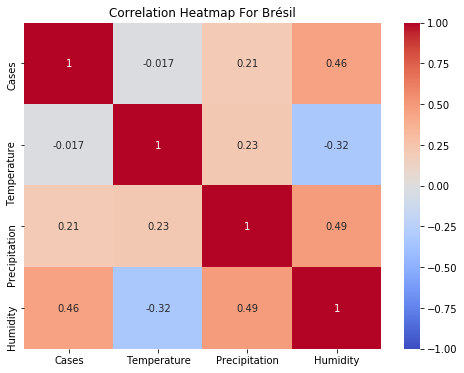
\includegraphics[width=0.5\linewidth]{figures/case_correlation}
			\vskip-0.5em
			\caption{Corrélation entre les variables climatiques et le nombre de cas}
		\end{figure}
	\end{frame}
	\begin{frame}{Exploration et Préparation des Données}
		\justifying
		\setstretch{1.2}
		\qquad La préparation des données pour le \textbf{Tchad} et le \textbf{Paraguay} a présenté des défis importants en raison du manque de données \textbf{suffisantes}.\\
		\pause[2]
		Pour pallier ces lacunes, nous avons envisagé plusieurs méthodes de traitement des données manquantes. Les méthodes sélectionnées sont les suivantes :
		\pause[3]
		\begin{itemize}
			\item \textbf{KNN Imputer} : Cette méthode utilise les k-plus proches voisins pour estimer les valeurs manquantes en se basant sur les données les plus proches.
			\pause[4]
			\item \textbf{Data  augmentation} ou \textbf{Augmentation de données} : est une technique utilisée pour augmenter artificiellement la taille d'un jeu de données en générant de nouvelles données à partir des données existantes.
		\end{itemize}
	\end{frame}
	\begin{frame}{Feature engineering}
		\justifying
		\setstretch{1.2}
		\qquad Le \textbf{feature engineering} est une technique qui consiste à créer de nouvelles variables (features) à partir des données brutes.\\
		\pause[2]
		\qquad Dans le cadre de notre étude, nous avons utilisé cette approche pour améliorer les données épidémiologiques du Brésil. En effet, lors de la collecte des données sur les cas de Chikungunya, nous avons rencontré un ensemble de données comprenant à la fois des patients testés positifs pour la dengue et pour le Chikungunya. Nous avons alors croisé les données des patients testés positifs par le Chikungunya avec les dates de détection de leur maladie. Cela nous a permis de créer une nouvelle variable (\textbf{feature}) associant chaque \textbf{cas} à une date spécifique, ce qui a enrichi notre base de données épidémiologiques.
	\end{frame}
	\begin{frame}{Feature engineering}
		\justifying
		\setstretch{1.2}
		Nous avons aussi utilisé de certaines technique :
		\pause[2]
		\begin{itemize}
			\justifying
			\item \textbf{Shifting} : Cette technique est particulièrement utile pour capturer les dépendances temporelles, car elle permet au modèle d'intégrer l'influence des valeurs passées sur les valeurs futures.
			\pause[3]
			\item  \textbf{Rolling} :  Cette technique est particulièrement utile pour réduire le bruit dans les séries temporelles, Cette méthode permet de lisser les fluctuations à court terme et de mettre en évidence les tendances ou cycles à plus long terme dans les données
		\end{itemize}
	\end{frame}
	\begin{frame}
		\begin{figure}
			\centering
			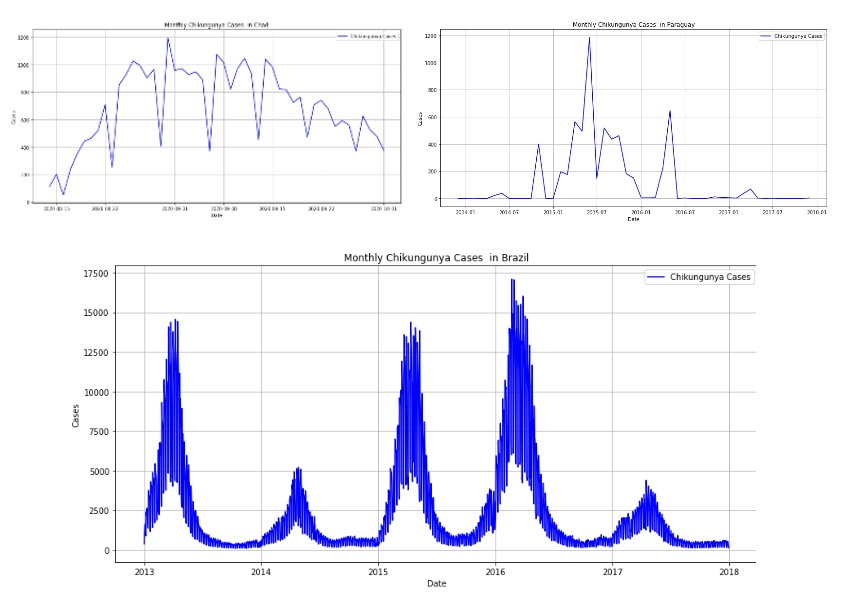
\includegraphics[width=0.72\linewidth]{figures/cases}
			\vskip-0.5em
			\caption{Visualisation numériques des cas du CHIKV au cours du temps dans les trois pays}
		\end{figure}
	\end{frame}
	\begin{frame}{Les métriques d’évaluation des modèles}
		\centering
		\setstretch{1.2}
		%\begin{block}{}
			\begin{tabular}{|c|l|}
				\hline
				\rule[-1ex]{0pt}{2.5ex}\textbf{Métrique} & \textbf{Formule mathématique} \\
				\hline
				\rule[-1ex]{0pt}{2.5ex} MAE(Erreur Absolue Moyenne) & $\text{MAE} = \frac{1}{n} \sum_{i=1}^{n} |y_i - \hat{y}_i|$ \\
				\hline
				\rule[-1ex]{0pt}{2.5ex} RMSE(Racine de l’Erreur Quadratique Moyenne) & $\text{RMSE} = \sqrt{\frac{1}{n} \sum_{i=1}^{n} (y_i - \hat{y}_i)^2}$ \\
				\hline
				\rule[-1ex]{0pt}{2.5ex} $R^{2}$ (Coefficient de détermination) & $R^2 = 1 - \frac{\sum_{i=1}^{n} (y_i - \hat{y}_i)^2}{\sum_{i=1}^{n} (y_i - \bar{y})^2}$ \\
				\hline
			\end{tabular}
		%\end{block}
	\end{frame}
	\begin{frame}
		\begin{figure}
			\centering
			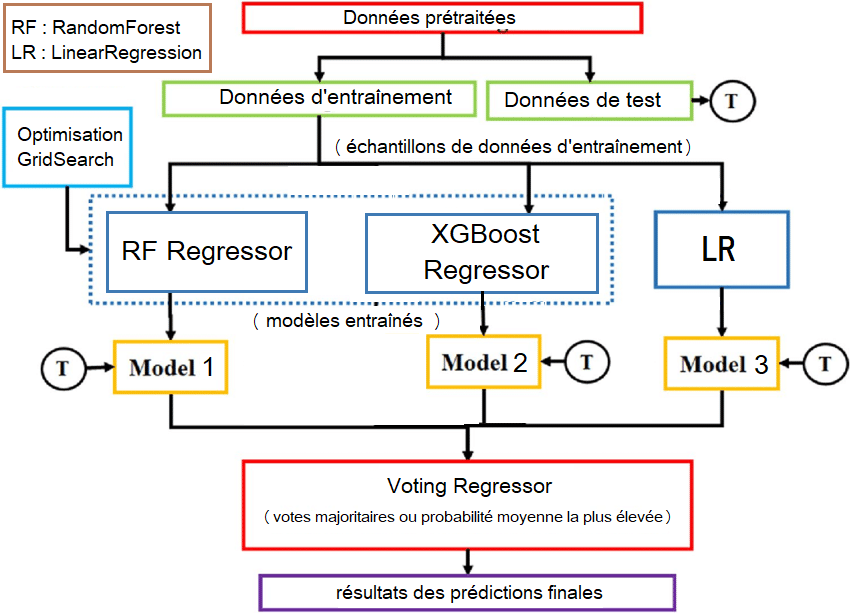
\includegraphics[width=0.72\linewidth]{figures/architecture}
			\vskip-0.5em
			\caption{Architecture de notre méthode}
		\end{figure}
	\end{frame}
	%------------------------------------------------
	% Section divider frame
	\makesection{Résultats et discussions}
	%------------------------------------------------
	%\begin{columns}
	%\begin{column}{0.45\textwidth}
	%  \colheader{Heading}
	%    \begin{enumerate}
		%        \item Statement
		%        \item Explanation
		%        \item Example
		%    \end{enumerate}
	%\end{column}
	%\begin{column}{0.45\textwidth}  %%<--- here
	%    \colheader{Heading}
	%    Lorem ipsum dolor sit amet, consectetur adipiscing elit. Integer lectus nisl, ultricies in feugiat rutrum, porttitor sit amet augue. Aliquam ut tortor mauris. Sed volutpat ante purus, quis accumsan dolor.
	%\end{column}
	%\end{columns}
	% Double columns
	\begin{frame}{Résultats et discussions}
		\begin{figure}
			\centering
			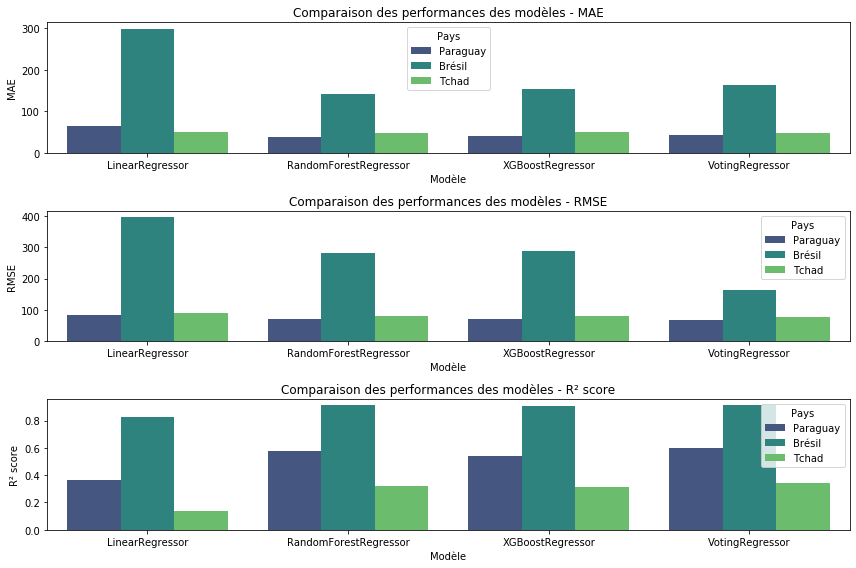
\includegraphics[width=0.6\linewidth]{figures/metric_comparaison}
			\vskip-0.5em
			\caption{Comparaison performance}
		\end{figure}
	\end{frame}
	\begin{frame}
		\begin{table}[!hbt]
			\centering
			\caption{Tableau de comparaison des différents modèles}
			\label{tab:performance}
			\begin{tabular}{|c|c|c|c|c|}	
				\hline
				Pays & Modèle & MAE & RMSE & R\textsuperscript{2} score \\
				\hline
				\multirow{4}{*}{Paraguay} & LinearRegressor & 65.4165 & 85.5322 & 0.3623 \\
				\cline{2-5}
				& RandomForestRegressor & 38.4501 & 69.9400 & 0.5736 \\
				\cline{2-5}
				& XGBoostRegressor & 40.4713 & 72.3494 & 0.5437 \\
				\cline{2-5}
				& \textbf{VotingRegressor} & \textbf{43.0001} & \textbf{68.1025} & \textbf{0.5957} \\
				\hline
				\multirow{4}{*}{Brésil} & LinearRegressor & 299.0416 & 396.7418 & 0.8229 \\
				\cline{2-5}
				& RandomForestRegressor & 141.0863 & 281.1369 & 0.9111 \\
				\cline{2-5}
				& XGBoostRegressor & 154.3493 & 288.9261 & 0.9061\\
				\cline{2-5}
				& \textbf{VotingRegressor} & \textbf{163.0350}  & \textbf{163.0350} & \textbf{0.9108} \\
				\hline
				\multirow{4}{*}{Tchad} & LinearRegressor & 51.5692 & 90.1886 & 0.1344 \\
				\cline{2-5}
				& RandomForestRegressor & 49.2575 & 79.7674 & 0.3229 \\
				\cline{2-5}
				& XGBoostRegressor & 51.1603 & 80.1259 & 0.3168 \\
				\cline{2-5}
				& \textbf{VotingRegressor} & \textbf{47.6738} & \textbf{78.5506} & \textbf{0.3434} \\
				\hline
			\end{tabular}
		\end{table}
	\end{frame}
	\begin{frame}
		\begin{figure}
			\centering
			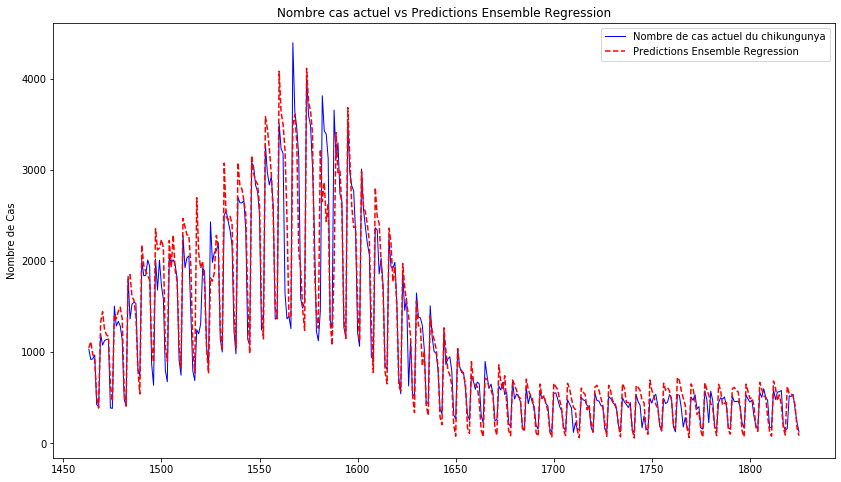
\includegraphics[width=0.75\linewidth]{figures/prediction_bresil}
			\vskip-0.5em
			\caption{Prédiction \textbf{Brésil} sur les ensembles de donnée de test avec notre modèle d'ensemble (\textbf{VotingRegressor})}
		\end{figure}
	\end{frame}
	\begin{frame}
		\begin{figure}
			\centering
			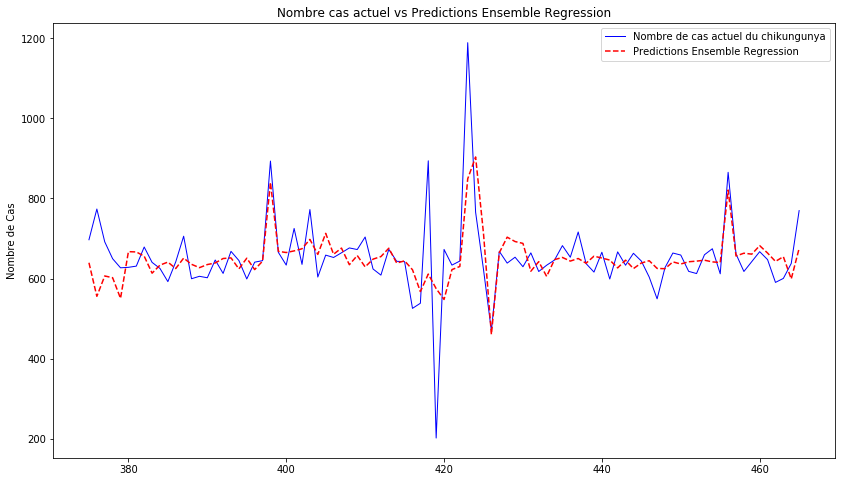
\includegraphics[width=0.75\linewidth]{figures/prediction_chad}
			\vskip-0.5em
			\caption{Prédiction \textbf{Tchad} sur les ensembles de donnée de test avec notre le modèle d'ensemble (\textbf{VotingRegressor})}
		\end{figure}
	\end{frame}
	\begin{frame}
		\begin{figure}
			\centering
			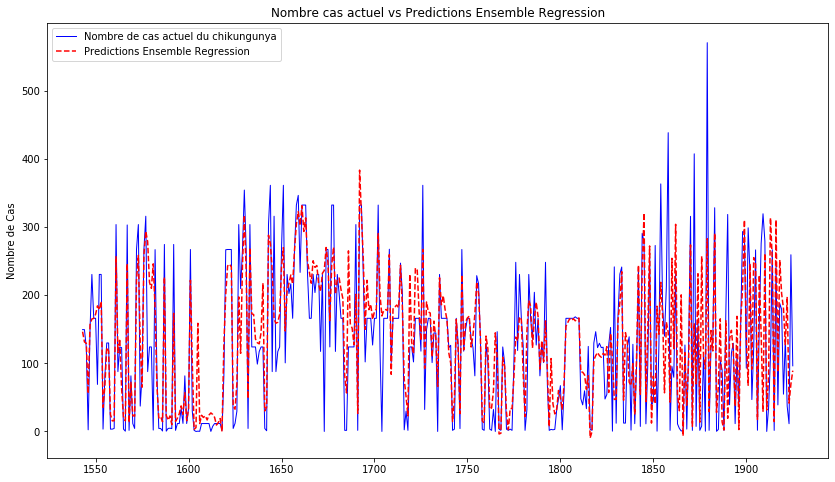
\includegraphics[width=0.75\linewidth]{figures/prediction_paraguay}
			\vskip-0.5em
			\caption{Prédiction \textbf{Tchad} sur les ensembles de donnée de test avec notre modèle d'ensemble (\textbf{VotingRegressor})}
		\end{figure}
	\end{frame}
	%------------------------------------------------
	% Section divider frame
	\makesection{Conclusion et perspectives}
	%------------------------------------------------
	% Table
	\begin{frame}{Conclusion et perspectives}
		\setstretch{1.2}
		\justifying
		\qquad L'objectif principal de cette étude était de Développer un modèle prédictif du chikungunya, en utilisant des approches de \textbf{régression d'ensemble}, en utilisant les variables climatiques. Les données épidémiologiques ont été obtenues sur le site du monitoring des cas d'épidomologie en temps réel \textbf{PAHO} (pour le Paraguay) ,dans le rapport d'\textbf{OMS}(pour le cas du Tchad) et dans le site \textbf{mendeley} pour celui du brésil tandis que les données climatiques provenaient de sources fiables telles que le site \textbf{WeatherAndClimate}. Les modèles choisis pour cette étude incluaient le \textbf{Random Forest Regressor} et le \textbf{XGBoost Regressor} optimisé via \textbf{Grid Search}, ainsi qu'un modèle d'ensemble (\textbf{Voting Regressor}) combinant \textbf{Linear Regression}, \textbf{Random Forest Regressor} et le \textbf{XGBoost Regressor} optimisé.
	\end{frame}
	\begin{frame}{Conclusion et perspectives}
		\vskip-2em
		\setstretch{1.2}
		\justifying
		Parmi ces modèles, notre modèle d'ensemble \textbf{Voting Regressor}, qui combine les prédictions des modèles \textbf{Linear Regression}, \textbf{Random Forest Regressor} et \textbf{XGBoost Regressor}, a affiché des performances globalement supérieures aux autres modèles individuels, avec un \textbf{MAE} minimal, un \textbf{RMSE} relativement bas et une très bonne précision (\textbf{91,08\%} pour le Brésil, \textbf{34,34\%} pour le Tchad et \textbf{59,57\%} pour le Paraguay).\\Les limites de l’étude ont montré que les variables climatiques ne suffisent pas à elles seules d'expliquer les variations des cas de chikungunya dans ces pays.\\[0.2cm]
		\begin{alertblock}{Perspectives}
			Intégrer d’autres facteurs environnementaux et de développer un modèle hybride pour améliorer les prévisions.
		\end{alertblock}
	\end{frame}
	
	
	%------------------------------------------------
	% Figure with wrapped text
	%\begin{frame}{Wrapped Figure}
	%    \begin{wrapfigure}{r}{0.4\textwidth}
		%    \centering
		%    \includegraphics[width=0.4\textwidth {figures/results_fig.pdf}
		%    \caption{Figure caption}
		%\end{wrapfigure}
		%"Lorem ipsum dolor sit amet, consectetur adipiscing elit, sed do eiusmod tempor incididunt ut labore et dolore magna aliqua. Ut enim ad minim veniam, quis nostrud exercitation ullamco laboris nisi ut aliquip ex ea commodo consequat. Duis aute irure dolor in reprehenderit in voluptate velit esse cillum dolore eu fugiat nulla pariatur. Excepteur sint occaecat cupidatat non proident, sunt in culpa qui officia deserunt mollit anim id est laborum.Sed ut perspiciatis unde omnis iste natus error sit voluptatem accusantium doloremque laudantium, totam rem aperiam.
		%\end{frame}
		
		%------------------------------------------------
		% Citations
		%\begin{frame}[fragile] % Need to use the fragile option when verbatim is used in the slide
		%    \frametitle{Citation}
		%    An example of the \verb|\cite| command to cite within the presentation:\\~
		
		%    This statement requires citation \cite{p1}.
		%\end{frame}
		
		%------------------------------------------------
		% Refenrenced
		\begin{frame}{Bibliographie}
			% Beamer does not support BibTeX so references must be inserted manually as below
			\footnotesize{
				\begin{thebibliography}{99}
					\bibitem[ECDC, 2024]{p1}{European Centre for Disease Prevention and Control (2024)\\
					Chikungunya worldwide overview\\ \url{https://www.ecdc.europa.eu/en/chikungunya-monthly}.
					}
					
					\bibitem[WHO, 2024]{p2}{World Health Organization (2024)\\
					Chikungunya worldwide overview\\ \url{https://www.who.int/health-topics/chikungunya\#tab=tab_1}.
					}
					\bibitem[CDC]{p3}{CDC: Transmission of chikungunya virus.\\
					\url{https://www.cdc.gov/chikungunya/php/
						transmission/index.html}}
					
					\bibitem[ResearchGate,2024]{p4}{Infographic showing transmission cycles of chikungunya virus(chikv)\\
					\url{https://www.researchgate.net/figure/Infographic-showing-transmission-cycles-of-chikungunya-virus-CHIKV-The-virus-is_fig3_339364587}}
					%            
					%            \bibitem[Doe, 2012]{p1} Joe Doe (2012)
					%            \newblock Title of the publication
					%            \newblock \emph{Journal Name} 12(3), 45 -- 678.
					%            \bibitem[Doe, 2013]{p} Jane Doe (2012)
					%            \newblock Title of the publication
					%            \newblock \emph{Journal Name} 12(3), 45 -- 678.
				\end{thebibliography}
				}

		\end{frame}
		
		\begin{frame}{Bibliographie}
		% Beamer does not support BibTeX so references must be inserted manually as below

		\footnotesize{
			\begin{thebibliography}{99}
				\bibitem[Springer,2023]{p5}{Study of the optimization control of agricultural greenhouse climatic parameters by the integration of machine learning figure on springer (2023).
					\url{https://link.springer.com/chapter/10.1007/978-3-031-43520-1_28}
				}
				\bibitem[Demanou,2010]{p6}{A retrospective serological and entomological survey (2010)\\Demanou, M., Antonio-Nkondjio, C., Ngapana, E., Rousset, D., Paupy, C., Manuguerra, J.C., Zeller, H.: Research article chikungunya outbreak in a rural area of western cameroon in 2006
				}
				%--
				
				\bibitem[Dr Jean,2020]{p7}{Dr Jean Bosco NDIHOKUBWAYO, D.B.H.e.a.: Rapport de la situation Épidémiologique chikungunya
				}
				
				\bibitem[Research Gate,2024]{p8}{The expansion of chikungunya in brazil-scientific figure on research-gate(2024). Available from :\url{https://www.researchgate.net/figure/Map-of-the-epicenters-of-chikungunya-cases-each-year-and-the-accumulated-cases-per_fig1_373336451}
				}

			\end{thebibliography}
		}
		\end{frame}
		%		, 
				\begin{frame}{Bibliographie}
			% Beamer does not support BibTeX so references must be inserted manually as below
			%
			\footnotesize{
				\begin{thebibliography}{99}
					\bibitem[Research Gate,2024]{p9}{Rapid epidemic expansion of chikungunya virus east/central/south african lineage , paraguay-scientific figure on research gate(2024).Available from:\\\url{https://www.researchgate.net/figure/Expansion-of-the-chikungunya-East-Central-South-African-lineage-epidemic-in-Paraguay-A_fig2_372620121}}
					
					\bibitem[IBM,2024]{p10}{What is ensemble learning?.Available from:\\\url{https://www.ibm.com/topics/ensemble-learning}}
					
					\bibitem[Roster K et Al,2022]{p11}{Machine-Learning-Based Forecasting of Dengue Fever in Brazilian Cities Using Epidemiologic and Meteorological Variables.\\Connaughton C, Rodrigues FA.  Am J Epidemiol. 2022 Sep 28;191(10):1803-1812. PMID: 35584963. doi: \url{10.1093/aje/kwac090}. }
					
					\bibitem[Rekha Gangula et Al,2023]{p12}{Ensemble machine learning based prediction of dengue disease with performance and accuracy elevation patterns. doi: \url{https://doi.org/10.1016/j.matpr.2021.07.270}. }
				\end{thebibliography}
			}
		\end{frame}
		%----------------------------------------------------------------------------------------
		% Final PAGE
		% Set the text that is showed on the final slide
		\finalpagetext{\centering MERCI POUR VOTRE AIMABLE ATTENTION ! ! ! !}
		%----------------------------------------------------------------------------------------
		\makefinalpage
		%----------------------------------------------------------------------------------------
	\end{document}